\documentclass[Main]{subfiles}
\begin{document}

\chapter{Elicitation Process}\label{cha:Elicitation}
\fxnote{skal skrives færdig}

This chapter describes the elicitation process carried out to create this requirement specification. In this chapter, "we" refers to the group of students carrying out the elicitation process.\\

Before starting the elicitation process, the costumer provided a short description of the tasks this new system is intended to support. This description helped us gain an initial understanding of the costumer's business goals.\\
 
The system described by this requirement specification is intended to be used by lecturers and students during the discrete math course. While not part of the elicitation process per se, we participated in said course, thus allowing us to observe the work process as users. Observing the work process contributed to our domain knowledge, by being exposed to the issues and problems of the current situation.\\

\begin{wrapfigure}{r}{0.6\textwidth}
\begin{center}
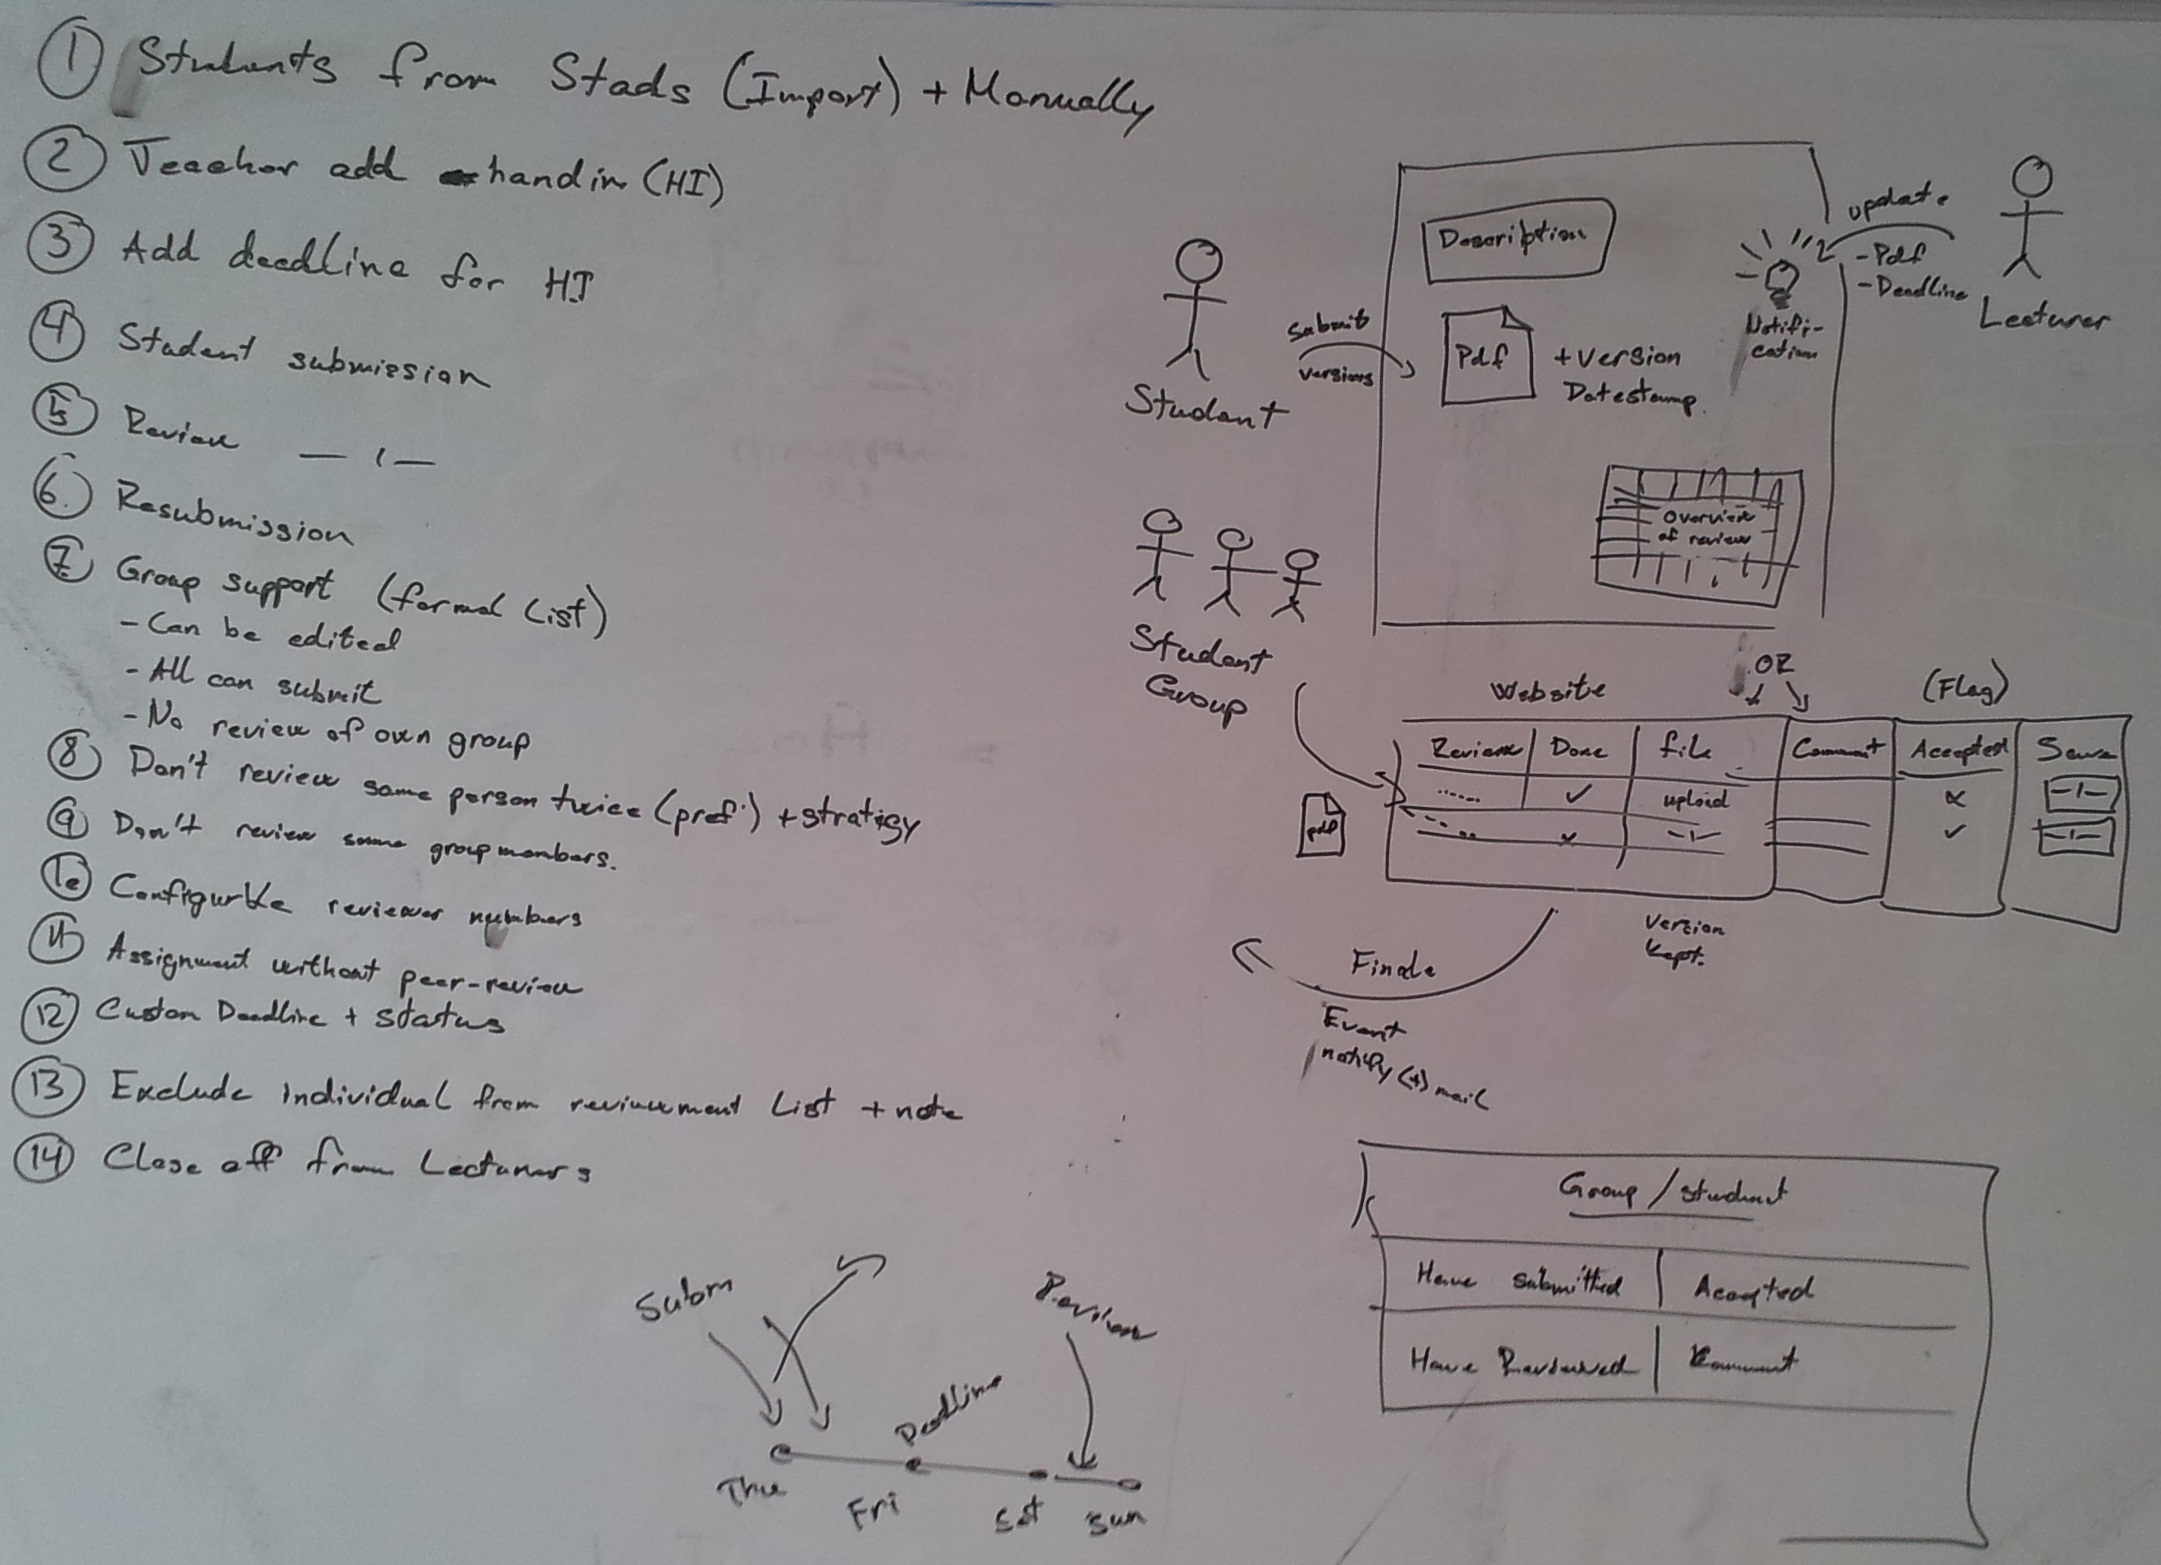
\includegraphics[width=0.58\textwidth]{IMG_20140221_131547.jpg}
\end{center}
\caption{Whiteboard notes created during user interview.}
\label{fig:UserInterviewNotes}
\end{wrapfigure}

To get an understanding of ... User interviews were conducted with the costumer. 
\\

Not used:
\begin{itemize}
\item Questionnaires - Was outside the scope of this project.
\item Brainstorm - New ideas was not needed.
\item Domain workshop - Not needed. The system was well-understood.
\item Focus group
\item Stakeholder analysis(implicit) - Finding the goal of the customer helped understand the system.
\end{itemize}




\end{document}